\documentclass[tikz,border=50mm]{standalone}
% !TeX program = luatex

%===This is the preambule I call in every file===

\usepackage{tikz}
\usepackage{xcolor}
\usepackage{pgfplots}
\usepackage{circuitikz}
\usepackage{tikz-3dplot}
\pgfplotsset{compat=newest}
\usetikzlibrary{arrows.meta, shapes.geometric, positioning, perspective, patterns.meta, decorations.pathreplacing, decorations.pathmorphing, decorations.markings, patterns, arrows.meta, shapes, shapes.geometric, decorations.text, angles, quotes,calc, 3d, math, circuits.ee.IEC,hobby, knots, intersections, through}


%=== The Euler Med Logo ===
%=== i.e. My signature ===

\usepackage{amsmath, amsfonts}
\makeatletter
\newcommand*\eulermed{{
\scalebox{3.3}{$\mathbb{E}$}\kern-1pt \scalebox{1.5}{u$\ell\varepsilon\rho$}\kern-55pt
\raisebox{19pt}{\scalebox{1.5}{$\mathcal{M}\varepsilon\delta$}}}
\@}
\makeatother

\begin{document}
%Simple pendulum
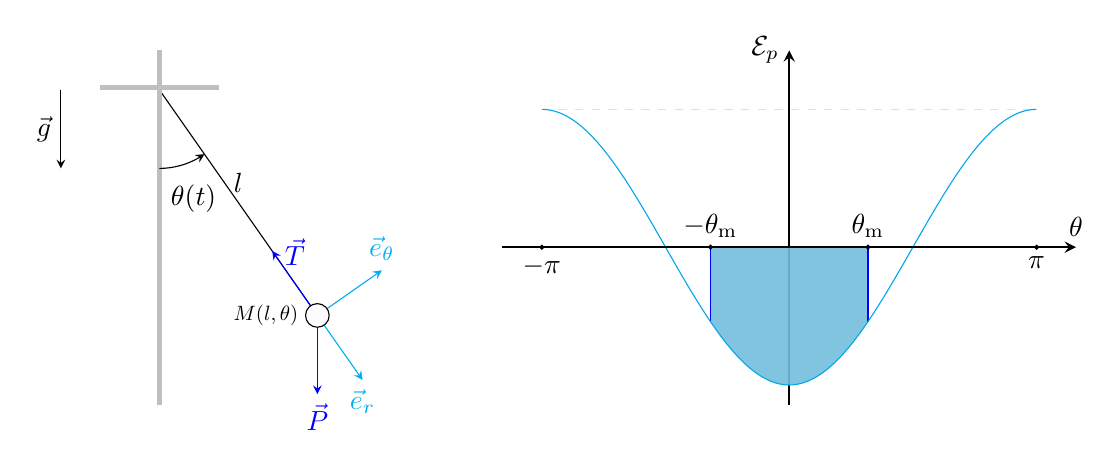
\begin{tikzpicture}[>=stealth]
\draw[->] (-1.25,0)--(-1.25,-1) node[midway, left] {$\vec{g}$}; 
%the support and the rod
\draw[smooth] (0,0)--(-55:3.5) node[midway, above] {$l$};
\draw[ultra thick, lightgray] (0,0.5)--(0,-4);
\filldraw[lightgray] (-0.75,0)rectangle(0.75,0.05);
%the angle theta 
\coordinate(o) at (0,0);
\coordinate(m) at (-55:3.5);
\coordinate(y) at (0,-2);
\pic[draw,->,inner sep=1pt, circle, draw,angle
eccentricity=1.45, "$\theta(t)$", angle radius = 10mm] {angle = y--o--m};
%The forces  and the polar base 
\draw[blue, ->] (-55:3.5)--(-55:2.5) node[above=0.1, midway] {$\vec{T}$};
\draw[cyan, ->] (-55:3.5)--(-55:4.5) node[below] {$\vec{e}_r$};
%Shifting the origin to the ball's coordinate
\begin{scope}[shift={(-55:3.5)}]
\draw[blue, ->] (0,0)--(0,-1) node[below] {$\vec{P}$}; 
\draw[cyan, ->] (0,0)--(35:1) node[above] {$\vec{e}_\theta$};
\draw[fill=white!95!lightgray] (0,0)circle(0.15) node[left=0.15, scale=0.75] {$M(l,\theta)$};
\end{scope}
%the energy graph 
\begin{scope}[shift={(8,-2)}]
\draw[smooth, dashed, white!50!lightgray] (-pi,1.75)--(pi,1.75);
\foreach \i/\j in {-pi/$-\pi$ , pi/$\pi$}{
\filldraw[] (\i,0)circle(0.025) node[below] {\j};
}
\draw[->, thick] (0,-2)--(0,2.5) node[left] {$\mathcal{E}_p$};
\fill[lightgray!50!cyan, opacity=0.9, domain=-1:1] (-1,0)--plot(\x,{-1.75*cos(\x r)})--(1,0)--cycle;

\draw[smooth, blue] (-1,0)--(-1,{-1.75*cos(1 r)});
\draw[smooth, blue] (1,0)--(1,{-1.75*cos(1 r)});
\draw[domain=-pi:pi, samples=500,cyan!95!blue] plot(\x,{-1.75*cos(\x r)});
\foreach \i/\j in {-1/$-\theta_\text{m}$ , 1/$\theta_\text{m}$}{
\filldraw[] (\i,0)circle(0.025) node[above] {\j};
}
\draw[->, thick] (-pi-0.5,0)--(pi+0.5,0) node[above] {$\theta$};
\end{scope}
\end{tikzpicture}
\end{document}
